\documentclass[11pt]{report}
\usepackage{amsmath,amsthm}
\usepackage{chngcntr}                                 
\theoremstyle{definition}
\newtheorem{example}{Example}
\counterwithin*{example}{chapter} 
\counterwithin*{example}{subsection} 
\theoremstyle{definition}
\newtheorem{q}{}
\counterwithin*{q}{chapter} 
\counterwithin*{q}{subsection} 
 \usepackage{booktabs}

\usepackage{multicol}
\usepackage[margin=1in]{geometry}
\usepackage{graphicx}
\graphicspath{{Graphics/}}

\author{Tarang Srivastava}

\usepackage{hyperref}
\hypersetup{
	colorlinks,
	citecolor=black,
	filecolor=black,
	linkcolor=black,
	urlcolor=black
}
\newcommand{\laplace}[1]{$ \mathcal{L}  \left\{ #1 \right\}$}
\newcommand{\laplaceMath}[1]{ \mathcal{L}  \left\{ #1 \right\}}
\newcommand{\laplaceMathInverse}[1]{ \mathcal{L}^{-1}  \left\{ #1 \right\}}
\newcommand{\laplaceMathComplete}[1]{ \mathcal{L}  \left\{ #1 \right\} = \int^\infty_0 e^{-st} #1 dt}
\newcommand{\diff}[2]{\dfrac{d #1}{d #2}}
\newcommand{\pdiff}[2]{\dfrac{\partial #1}{\partial #2}}
\newcommand{\sdiff}[2]{\dfrac{d^2 #1}{d {#2}^2}}
\newcommand{\putpic}[1]{
		\centering
		\includegraphics[width=10cm]{#1}
}
\newcommand{\heaviside}[1]{u_{#1} (t)}
\begin{document}
	
	\begin{titlepage}
		\begin{center}
			\vspace*{1cm}
			\Huge
			\textbf{Differential Equations}\\
			\vspace{0.5cm}
			\LARGE
			A Concise Review of Elementary Differential Equations\\
			\vspace{1.5cm}
			\textbf{Tarang Srivastava}\\
			\vfill
			\vspace{0.8cm}
			\Large
			Dr. Mesut \c{C}akir\\
			Differential Equations and Complex Analysis\\
			South Brunswick High School\\
			14 February 2018
		\end{center}
	\end{titlepage}
	
	\tableofcontents	
	\pagebreak
	
	\chapter{Introduction}
\section{Basic Mathematical Models}
In this concise review we will provide brief explanations to the core concepts of differential equations, and include some examples to show the many techniques used in differential equations. Refer to the scratch paper if further examples and procedures are needed. For future reference the textbook used is "Elementary Differential Equations and Boundary Value Problems" by William E. Boyce and Richard C. DiPrima. All the graphics used in this document were created by Tarang Srivastava in Wolfram Mathematica \\

Equations considering derivatives are \textbf{differential equations}. A differential equation that describes a physical process is a \textbf{mathematical model}. \\
A model for an object falling in earth's atmosphere may be given by the differential equation $m \frac{dv}{dt} = mg - \gamma v$. Moving things around we get $\frac{dv}{dt} = 9.8 - \frac{v}{5}$ There are several solutions for this equation and can be represented by the slope field. \\
\begin{center}
	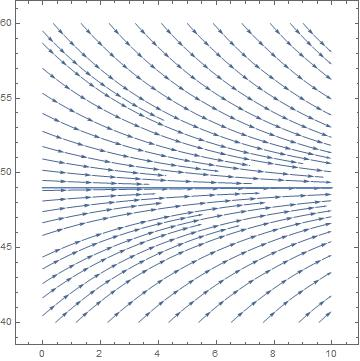
\includegraphics[width=7cm]{f1}
	$$\frac{dv}{dt} = 9.8 - \frac{v}{5}$$
\end{center}
The line $y=49$ shows the equilibrium solution for this case\\
\section{Solutions of Differential Equations}
When a problem is given where there are infinite solutions, usually when there is a constant in the solution as a result of integration, an \textbf{initial condition} can be set to find a particular answer, this is called an \textbf{initial value probelm}. A general example of this is
\begin{align*}
\dfrac{dy}{dt} = ay - b \\
y(0) = y_0 \\
\frac{dy/dt}{y-(b/a)} = a\\
\ln{ \vline y-(b/a) \vline} = at + C && \text{Where C is an arbitrary constant}\\ 
y = b/a + ce^{at} && \text{solve for C using the initial condition}\\
y = b/a + (y_0 - b/a)e^{at}
\end{align*}
The \textbf{general solution} with the constant gives all possible solutions, and graphs the \textbf{integral curves} 
\begin{center}
	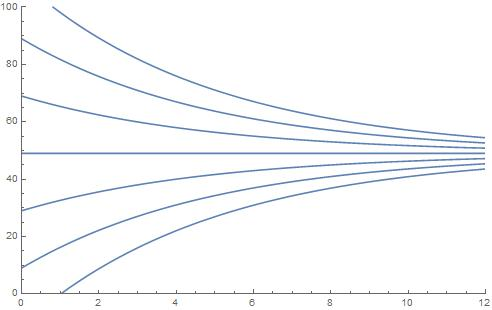
\includegraphics[width=12cm]{f2}
\end{center}
$$v = 49 + ce^{-t/5}$$
\section{Classification of Differential Equations}
Differential equations are classified into \textbf{ordinary differential equations} and \textbf{partial differential equations}. ODE have ordinary derivatives whereas PDE have partial derivatives. The \textbf{order} is the highest derivative. There are linear and nonlinear functions, we will mostly deal with linear for now. 
\pagebreak
\section{Chapter 1 Assessment}
\begin{multicols*}{2}
	\begin{enumerate}
		\item Consider the equation $\diff{p}{t} = 0.5p -450$ that gives the population of a certain species
		\begin{enumerate}
			\item Find the general solution to this equation
			\item Solve for the equilibrium solution 
			\item Solve for the specific solution if there are initially 1000 members in the species
		\end{enumerate}
		\item Consider the equation $\diff{y}{t} = ay - b$
		\begin{enumerate}
			\item Find the general solution
			\item Solve the initial value problem for $y(0) = y_0$
		\end{enumerate}
		\item Consider the equation $\diff{y}{t} + 2y = 3$ 
		\begin{enumerate}
			\item Find the integrating factor, $\mu(t)$ 
			\item Find the general solution 
			\item State the equilibrium solution 
		\end{enumerate}
		\item Show the solution for the arbitrary equation $\diff{y}{t} + ay = g(t)$ in terms of a general integral solution. 
		\item Solve the initial value problem for $ty' + 2y = 4t^2$ with the value $y(1) = 2$ 
		\item Solve the differential equation $\diff{y}{t} - 2y = 4 -t$, find the initial point that separates solutions that grow large positively to large negatively when $t\rightarrow \infty $ 
		\item Given the equation $\diff{p}{t} = 0.5p - 450$ that gives the population of a species (t = months)		\begin{enumerate}
			\item Find the time the population becomes extinct if $p(0) = 850$
			\item Find the time of extinction if $p(0) = p_0$ where $0 < p_0 < 900$
			\item Find the initial population if the population becomes extinct after 1 year 
		\end{enumerate}
	\end{enumerate}
\end{multicols*}
	\chapter{First Order Differential Equations}
We will focus on differential equations of first order 
$$\diff{y}{t} = f(t,y)$$
One of the notations used is that for any differentiable function $y=\phi(t)$ that satisfies the differential equation. 
\section{First Order Linear Equation}
$$P(t) \diff{y}{t} + Q(t)y = G(t)$$
This gives a standard form for solving linear equations. To solve such linear equations, we use a \textbf{integrating factor} $\mu(t)$. \\
\begin{example}
	Find the general solution of the differential equation
	\begin{align}
	\diff{y}{t} + \frac{1}{2} y = \frac{1}{2}e^{t/3} \\
	\mu(t)\diff{y}{t} + \mu(t)\frac{1}{2} y = \mu(t)\frac{1}{2}e^{t/3} && \text{we multiply by the integrating factor} \\
	\diff{}{t}[\mu(t)y] = \mu(t)\diff{y}{t} + \diff{\mu(t)}{t} y && \intertext{We notice that the first part on the right side of (3) exists as the first part in (2)}\\
	\diff{\mu(t)}{t} = \frac{1}{2} \mu(t)\\
	\frac{d\mu(t)/dt}{\mu(t)} = \frac{1}{2}\\
	\diff{}{dt} \ln \vline \mu(t) \vline = \frac{1}{2}\\
	\ln \vline \mu(t) \vline = \frac{1}{2}t + C && Integrating follows\\
	\mu(t) = c e^{t/2} && \intertext{Any value for c (obviously not 0) can be used to find the integrating factor. Since there are multiply integrating factors that would suffice, so we use $c = 1$} \\
	e^{t/2}\diff{y}{t} + \frac{1}{2}e^{t/2}y = \frac{1}{2}e^{5t/6} \\ 
	\diff{}{t} \left( e^{t/2} y\right) = \frac{1}{2}e^{5t/6} && \text{This was the whole point of using $\mu(t)$}\\
	\left( e^{t/2} y\right) = \frac{3}{5}e^{5t/6} + c && \text{from integrating both sides}\\
	y = \frac{3}{5}e^{t/3} + ce^{-t/2} && \text{Solving for y}\\
	\intertext{This is the general solution. Huzzah! Lets say we have to find a solution that goes through point (0,1) then we solve for c by setting $y=1$ and $t=0$}
	y = \frac{3}{5}e^{t/3} + \frac{2}{5}e^{-t/2} && \text{This is also the initial value solution}
	\end{align}
\end{example}


\begin{center}
	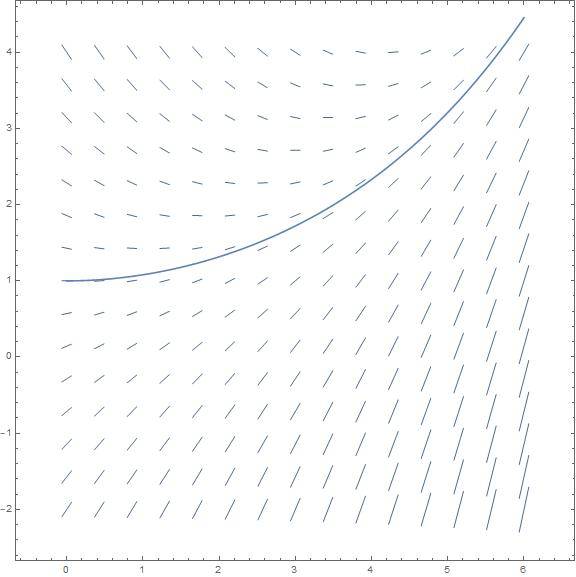
\includegraphics[width=10cm]{f3}\\
	Here is a graph of the slope field(1) and the initial value solution(15). 
\end{center}
\section{Separable Equations}
These are generally the easiest differential equations to solve, as they require a simple rearrangement and then integration. Though you should consider possibly the intervals in which a solution exists, especially when you are given an initial value condition, since you may obtain two (or more) general solution and you have to find the one that contains the initial value. \\
Separable equations are equations of the form $$M(x) dx + N(y)dy = 0$$ 
\begin{example} Solve the initial value problem, and determine the interval in which the solution exists. 
	\begin{align*}
	\diff{y}{x} = \frac{3x^2+4x+2}{2(y-1)}, && y(0) = -1 
	\intertext{The equation can be rewritten as}
	2(y-1)dy = (3x^2+4x+2)dx 
	\intertext{Integrating the left side with respect to y, and the right side with respect to x}
	y^2-2y = x^3 + 2x^2 +2x+c 
	\intertext{solving for c using the initial coniditon $x=0$ and $y=-1$ and get $c = 3$. The solving for y in terms of x, we complete the square and find}
	y = 1 \pm \sqrt{x^3 + 2x^2 + 2x+4} 
	\intertext{considering the initial value condition only the $	y = 1 - \sqrt{x^3 + 2x^2 + 2x+4}$ satisfies the conidition }
	\end{align*}
\end{example}


%	\subsection{Modeling with First Order Equations}
This should be an important focus on anyone trying to learn Differential Equations, and effectively use it. Personally, I believe this is the hardest part and the most useful part of this subject. We will study several examples that deal with modeling, and there are a couple of basic tricks we will understand when learning to model differential equations. 
\begin{example}
	%		 
	At time $t = 0$ a tank contains $Q_0$ lb of salt dissolved in 100 gal of water; Assume that water containing $\dfrac{1}{4}$ lb of slat/gal is entering the tank at a rate of $r$ gal/min, and that well-stirred mixture is draining from teh tank at the same rate. Set up the initial value problem that describes this flow process. Find the amount of salt $Q(t)$ in the tank at any time, and also find the limiting amount $Q_L$ that is present after a very long time. If $r=3$ and $Q_0=2Q_L$, find the time $T$ after which the salt level is within $2\%$ of $Q_L$. Also find the flow rate required if the value of $T$ is not to exceed 45 min.\\ \begin{center}
		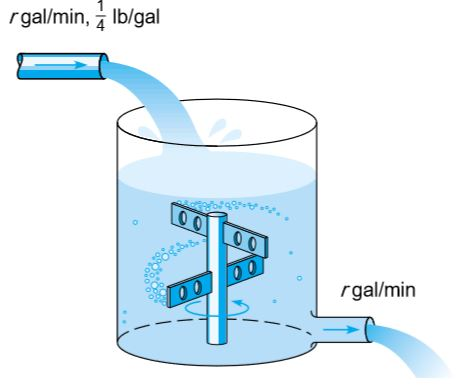
\includegraphics[width=10cm]{figure231} 
	\end{center} 
	\begin{multicols}{2}
		\begin{align}
		\diff{Q}{t} = \text{rate in} - \text{rate out} 
		\intertext{salt enters at  $\dfrac{1}{4}$ lb/gal times the flow rate $r$ gal/min. Also volume is constant, and concentration is uniform}
		\diff{Q}{t} = \dfrac{r}{4} - \dfrac{rQ}{100}
		\intertext{The initial condition is}
		Q(0) = Q_0
		\intertext{rearragning to}
		\diff{Q}{t} = \dfrac{rQ}{100} = \dfrac{r}{4}
		\intertext{solving for the genral solution with the integrating factor $e^{rt/100}$ we find}
		Q(t) = 25 + ce^{-rt/100}
		\intertext{Using the initial condition we find the initial solution to be}
		Q(t) = 25 + (Q_0-25)e^{-rt/100}
		\intertext{$Q(t) \rightarrow 25 $ as $t \rightarrow \inf$ so the limiting value} 
		Q_L = 25
		\end{align}
	\end{multicols}
	\begin{figure}[h]
		\centering
		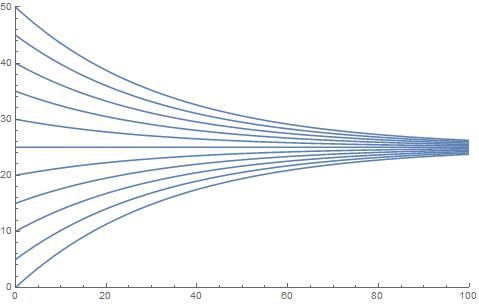
\includegraphics[width=10cm]{Model1}
		\caption{Several plots for the general solution (20) for Example 3}
		Considering Figure 1 we see that the values converge to 25, which supports that $Q_L = 25$
	\end{figure}
	
\end{example}
In the previous example te rate in and out did not vary, we will consider a similar example in which it does vary. This does not make the problem more difficult, but we will study this behavior in the graph of the initial solution. 
\begin{example}
	
	Consider a pond that initially contains 10 million gal of fresh water. Water containing an undesirable chemical flows into the pond at the rate of 5 million gal/year and the mixture in the pond flows out into the pond at the rate of 5 million gal/year and the mixture in the pond flows out at the same rate. The concentration $\gamma (t)$ of chemical in the incoming water varies periodically with time according to the expression $\gamma(t) = 2 + \sin 2t g/gal$. Construct a mathematical model of this flow process and determine the amount of chemical in the pond at any time. Plot the solution and describe in words the effect of the variation in the incoming concentration. Since the incoming and outgoing flows of water are the same, the amount of water int eh pond remains constant at $10^7$ gal. Let us denote time by $t$, measured in years, and the chemical by $Q(t)$, measured in grams. This example is similar to Example 1 and the same inflow/outflow principle applies. 
	\begin{align*}
	\diff{Q}{t} = \text{rate in} - \text{rate out}, \\
	\text{rate in} = (5 \times 10^6)(2+\sin 2t) 
	\intertext{The concentration of chemical in the pond is $Q(t)/10^7$, so the rate of flow out is}
	\text{rate out} = (5 \times 10^6)(Q(t)/10^7) = Q(t)/2 \\
	\diff{Q}{t} = (5 \times 10^6)(2 + 2\sin 2t )- \dfrac{Q(t)}{2} 
	\intertext{to make the work more easy lets introuduce $q(t) = Q(t)/10^6$}
	\diff{q}{t} + \dfrac{1}{2}q = 10 + 5 \sin 2t
	\intertext{the initial condition is}
	q(0) = 0 
	\intertext{the integrating factor is $e^{t/2}$}
	q(t) = 20-\dfrac{40}{17}\cos 2t + \dfrac{10}{17} \sin 2t + ce^{-t/2}
	\intertext{solving for the initial condition}
	q(t) = 20-\dfrac{40}{17}\cos 2t + \dfrac{10}{17} \sin 2t - \dfrac{300}{17}e^{-t/2}
	\end{align*}
	\begin{figure}[h]
		\centering
		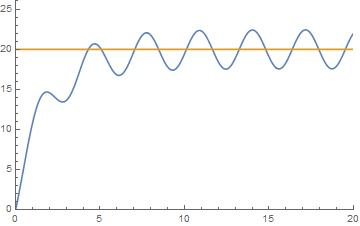
\includegraphics[width=10cm]{Model2}
		
	\end{figure}
	
\end{example}
\pagebreak
\section{Differences Between Linear and Nonlinear Equation}
Let the functions of $f$ and $\partial f / \partial y$ be continuous in some rectangle $\alpha < t < \beta$, $\gamma < y < \delta$ containing the point $(t_0,y_0)$. Then in some interval $t_0-h<t<t_0+h$ contained in $\alpha < t < \beta $, there is a unique solution $y=\phi (t)$ of an initial value problem
\begin{example}
	Find the interval of the initial value problem 
	\begin{align*}
	ty' + 2y = 4t^2 \\
	y(1) = 2 \\
	y' = (2/t)y = 4t 
	\intertext{Referring to the form $y' + p(t)y = g(t)$ we find that $p(t) = 2/t$ and $g(t) = 4t$. $g(t)$ is continuous everywhere but $p(t)$ is only continuous in $(-\infty, 0)\cup (0,\infty)$ Since the ininitial value gives that $y(1) = 2$, we know that the equation exists in the interval, and has a unique solution}
	y = t^2 + \dfrac{1}{t^2}, && t>0
	\end{align*}
\end{example}
%	\subsection{Autonomous Equations and Population Dynamics}
We will consider a specific example on how to derive the equation for carrying capacity, and population dynamics of a species
\begin{align*}
dy/dt = f(y) && \text{This is the form we will consider} \\
dy/dt = ry 
\intertext{if we subject it to an initial condition}
y(0) = y_0 \\
y = y_0 e^{rt}
\intertext{Now to actually show that growth rate depends on population, we get}
dy/dt = h(y)y && \text{Replacing $r$ with $h(y)$} \\
dy/dt = (r-ay)y 
\intertext{This represents the population growth. We rewrite it as}
\diff{y}{t} = r\left( 1 - \dfrac{y}{K}\right)y && \text{Where $K = r/a$}
\intertext{The simplest form is where growth is constant so $dy/dt = 0$. This gives}
r(1-y/K)y = 0
\intertext{This gives the two equilibrium solutions}
y = \phi _1 (t) = 0 \\
y = \phi _2 (t) = K 
\intertext{Using techniques in the earlier sections we can find the solution to when the growth rate is not constant. We separate the earlier equation and get}
\dfrac{dy}{(1-y/K)y} = r dt
\intertext{Use partial fraction seperation}
\left( \dfrac{1}{y} + \dfrac{1/K}{1-y/K}\right)dy = rdt
\intertext{Integrate both sides}
\ln |y| - \ln |1-\dfrac{y}{K}| = rt + c
\intertext{Solving for y, and the constant we get}
y = \dfrac{y_0K}{y_0 + (K-y_0)e^{-rt}} && \text{This is the solution for such a differential equation}
\end{align*}
\section{Exact Equations and Integrating Factors}
This is fun. We will discuss another method for solving first order differential equations in very special cases 
\begin{example}
	Solve the differential equation
	\begin{align*}
		2x + y^2 +2xyy' = 0
		\intertext{Here we realize that if we have a function $ \psi (x,y) = x^2 + xy^2 $ it has the property that}
		2x+y^2 = \pdiff{\psi}{x}, && 	2xy = \pdiff{\psi}{y}
		\intertext{We can rewrite it as}
		\pdiff{\psi}{x} + \pdiff{\psi}{y} \dfrac{dy}{dx}
		\intertext{Here we make an important assumption. We assume that $y$ is a function of $x$, so we can use the chain rule}
		\pdiff{\psi}{x} = \diff{}{x} (x^2+xy^2) = 0 \\
		\intertext{And then we integrate for the solution}
		\psi(x,y) = x^2 + xy^2 = c 
	\end{align*}	
\end{example}
Now we will consider how to solve for $N(x,y)$ and $M(x,y)$ and then use that to solve for the differential equation. 
\begin{example}
	Solve for the differential equation $ (y \cos x + 2xe^y ) + (\sin x + x^2 e^y -1)y' = 0 $
	\begin{gather*}
		M(x,y) = y \cos x + 2xe^y \\
		N(x,y) = \sin x + x^2 e^y -1 \\
		\intertext{Taking the appropriate partial derivative gives}
		M_y= \cos x + 2xe^y \\ N_x = \cos x + 2xe^y
		\intertext{This shows that an exact solution exists that will satisfy both the equations}
		\pdiff{\psi}{x} = y \cos x + 2xe^y 
		\intertext{Which integrating gives}
		\psi = y \sin x + x^2e^y + h(y)
		\intertext{We use $h(y)$ for any constant $c$. Solving for the $N(x,y)$ we get }
		\pdiff{\psi}{y} = \sin x + x^2 e^y + h'(y) = N_x = \sin x + x^2 e^y - 1 \\
		\int h'(y) = \int -1 dy \\
		h(y) = -y + c\\
		y \sin x + x^2e^y - y = c
	\end{gather*}
\end{example}
\pagebreak
\section{Chapter 2 Assessment}
\begin{multicols*}{2}
	\begin{enumerate}
		\item Solve for the general solution 
		$$\diff{y}{x} = \dfrac{x^2}{1-y^2}$$
		\item $ (4+t^2) \diff{t}{t} + 2ty = 4t$
		\begin{enumerate}
			\item Solve the general solution
			\item Solve for when $y(0) = 3$ 
		\end{enumerate}
		\item Follow all the steps to receive full credit $$\diff{y}{t} + \dfrac{1}{2} y = \dfrac{1}{2}e^{t/3}$$ 
		\begin{enumerate}
			\item Give the general solution for $\mu(t)$
			\item Find the general solution of the equation
			\item Find the solution passing through (0,1)
		\end{enumerate}
		\item Find the general solution for 
		$$\diff{y}{t} + p(t)y	 = g(t)$$
		\item Solve initial value problem 
		\begin{align*}
		ty' + 2y = 4t^2 \\
		y(1) = 2
		\end{align*}
		\begin{enumerate}
			\item State the integrating factor
			\item Solve for the general solution
			\item Solve for the initial condition
			\item State the boundaries for the solution
			\item Show where the solutions do not exist 
		\end{enumerate}
		\item Solve the initial value problem for when $y(0) = -1$
		$$\diff{y}{x} = \dfrac{3x^2+4x+2}{2(y-1)}$$
		\begin{enumerate}
			\item Solve for the implicit general solution
			\item Show the implicit solution
			\item Solve for all solution for y
			\item State the particular solution 
		\end{enumerate}
		\item Suppose that a sum $S_0$ is invested at an annual rate of return r compounded 	continuously 
		\begin{enumerate}
			\item Find the time T required for the original sum to double in value as a function of r
			\item Determine T if $r = 7$
			\item Find the return rate that must be achieved if the initial investment is to double in 8 years 
		\end{enumerate}
		\item Solve the following differential equation
		$$ 2xy - 9x^2 + (2y + x^2 + 1) \diff{y}{x} = 0 $$
		\item Solve the following initial value problem for $y(-1) = 8$
		$$2xy^2+4=2(3-x^2y)y'$$
		\item Solve the differential equation 
		$$(y\cos x + 2xe^y) + (\sin x + x^2 + x^2e^y-1)y' = 0 $$
		\item Solve the differential equation 
		$$ (3xy+y^2) + (x^2+xy)y' = 0$$
		\begin{enumerate}
			\item Show whether the equation is exact
			\item Solve for the integrating factor
			\item State the general solution
		\end{enumerate}
		\item Arrive at this solution, that is used to find the integrating factor. Assume that $\mu$ is only a function of $x$
		$$\diff{\mu}{x} = \dfrac{M_y-N_x}{N} \mu$$
		\item An investor depositis \$1000 in an account paying interest at a rate of 8\% compounded monthly, and also makes additional deposits of \$25 every month. Find the balance in the account after 3 years
	\end{enumerate}
\end{multicols*}

	\chapter{Second Order Differential Equations}
\section {Introduction}
A general form we will use for second order linear equations 
$$P(t) y'' + Q(t)y' + R(t)y = G(t)$$
If we divide it out by $ P(t) $ we get another form that is useful in solving these equations. 
\[ y'' + p(t)y' + q(t)y = g(t) \]
A second linear equation can be specified as being \textbf{homogeneous} if the $ g(t) $ or the $ G(t) $ term is 0. Thus \textbf{nonhomogeneous} is when this is not the case. It is much easier to solve when the coefficients are constants. 
\section{Homogeneous Equations with Constant Coefficients}
	Second order ordinary differential equation follows the form $$\sdiff{y}{t} = f \left(t, y, \diff{y}{t} \right) $$
	\begin{example}
		Find the general solution of $y'' + 5y' + 6y = 0$
		\begin{gather*}
			\intertext{We start by assuming that y is of some form $e^{rt}$}
			(r^2+5r+6)e^{rt} = 0 \\
			(r+2)(r+3) = 0\\
			r_1 = -2\\	r_2=-3
			\intertext{This gives the general solution}
			y = c_1 e^{-2t} + c_2 e^{-3t}
		\end{gather*}
		Note that the solution is a linear combination of two $e^{rt}$ combinations. Also there are two constants and in order to solve the two constants you need both the initial value, and an initial slope. Lets consider the same example with initial values $y(0) = 2$ and at that point the slope = -1
		\begin{align*}
			\intertext{The two inital conditions are essentially}
			y(0) = 2 && y'(0) = -1 
			\intertext{Solving for the initial condition we get the two equations}
			2 = c_1 + c_2 && -1 = -2c_1 - 3c_2
		\end{align*} 
		The solutions are $c_1 = 5$ and $c_2 = -3$ giving the particular solution as $y = 5e^{-2t} - 3e^{-3t}$
	\end{example}

	The previous example introduces us to the idea of second order differential equations, and how one would go about solving a simple problem like that. Now lets consider the more general equation 
	\[ ay'' + by' + cy = 0 \]
	Note that this is a homogeneous equation with constant coefficients. We will begin by assuming that the function $ y $ is of some for $ e^rt $. following this assumption we find that 
	\begin{align*}
		\intertext{if $ y = e^rt $ then}
		y' = re^{rt} && y'' = r^2e^{rt}
	\end{align*}
	replacing the values in the original equation we get
	\[ 	ar^2e^{rt} + bre^{rt} + ce^{rt} = 0 \]
	At this point it should be clear that we can factor out $ e^rt $ and since it is never 0, the resulting equation must be equal to 0. Note that it is also a quadratic, so now it is basically an Algebra 1 problem
	\[ (ar^2 + br + c)e^{rt} = 0 \]
	The previous equation is called the \textbf{characteristic equation}. Lets consider the usefulness of the characteristic equation. 
	\begin{example}
		Find the solution of the initial value problem
		\[ 4 y'' - 8y' + 3y = 0 \]
		with initial values $ y(0) = 2 $, and $ y'(0) = \dfrac{1}{2} $\\
		If we assume that $ y $ is a function of the form $ e^{rt} $ then the characteristic equation is 
		\[ 4r^2 - 8r+3 = 0 \]
		The roots are then $ r = 3/2 $ and $r = 1/2$ therefore the general solution is
		\[ y = c_1 e^{3t/2} + c_2 e^{t/2} \]
		This gives the two solutions 
		\begin{align*}
			c_1 + c_2 = 2, && \dfrac{3}{2} c_1 + \dfrac{1}{2}c_2 = \dfrac{1}{2}
		\end{align*}
		Which gives the two values $ c_1 = -\dfrac{1}{2} $ and $ c_2 = \dfrac{5}{2} $ and the particular solution
		\[ y =  -\dfrac{1}{2}e^{3t/2} + \dfrac{5}{2}e^{t/2}\]
	\end{example}
\section{The Wronskian}
Lets start by considering the general form of a second order linear differential equation
\[ ay'' + by' + c = 0 \]
Now lets consider a differential operator, denoted $ L $ that will give such results
\[ L[y] = y'' + p(t)y' + q(t)y = 0 \]
The initial values for the operator are also considered 
\begin{align*}
	y(t_0) = y_0, && y'(t_0)=y'_0
\end{align*}
lets consider the \textbf{Existence and Uniqueness Theorem} which states
\begin{align*}
	\intertext{Consider the initial value problem}
	y''+p(t)y' + q(t)y = g(t), && y(t_0) = y_0,&& y'(t_0) = y'_0
\end{align*}
where $ p $, $ q $ and $ g $ are continuous on an open interval $ I $ that contains the point $t_0$ then there is exactly one solution $ y = \phi(t)  $ of this problem, and the solution exists throughout the interval $ I $ \\
\\
This theorem says three main things
\begin{enumerate}
	\item The initial value problem \textit{has} a solution; in other words, a solution \textit{exists}
	\item The initial value problem has \textit{only one} solution; that is, the solution is unique
	\item The solution $ \phi $ is defined \textit{throughout the interval I} where the coefficients are continuous and is at least twice differentiable there.  
\end{enumerate}
\begin{example}
	Okay, I know you did not understand any of that before. So consider this example
	\begin{align*}
		\intertext{Find the longest interval in which the solution of the initial value problem exists. }
		(t^2-3t)y'' + ty' - (t+3)y = 0, && y(1)=2, && y'(1)=1
		\intertext{is certain to exist.}
		\intertext{We begin by solving this by first making it follow the form in the theorem}
		y'' + \dfrac{t}{y^2+3t}y' - \dfrac{t+3}{t^2-3t}y = 0
	\end{align*}
	\begin{align*}
	\intertext{This follows}
		g(t) = 0, && p(t) = \dfrac{t}{y^2+3t}, && q(t)= -\dfrac{t+3}{t^2-3t}
	\intertext{Which gives that $t \ne 3$ and $ t \ne 0 $. therfore splitting $ I $ into three separate intervals. Since 1 is less than but greater than 3 and 0, the interval for $ I $ is}
	0<t<3
	\end{align*}
\end{example}
Lets consider the \textbf{Principle of Superposition}. If $ y_1 $ and $ y_2 $ are two solutions of the differential equation
\[ L[y] = y'' + p(t)y' + q(t)y = 0 \]
Then the linear combination of $ c_1 y_1 + c_2 y_2 $ is also a solution.\\
If the previous statement is true, that means it must satisfy the condition $ L[y] = 0 $.
\begin{align*}
	L[c_1 y_1 + c_2 y_2 ] &= [c_1 y_1 + c_2 y_2 ]'' + p[c_1 y_1 + c_2 y_2 ]' + q[c_1 y_1 + c_2 y_2 ] = 0 \\
	&= c_1y_1'' + c_2y_2'' + c_1y_1' + c_2y_2' + c_1y_1 + c_2y_2 \\
	&= c_1[y_1'' + y_1' + y_1] + c_2[y_2'' + y_2' + y_2]\\
	&= c_1L[y_1] + c_2L[y_2]
\end{align*}
Since $ y_1 $ and $ y_2 $ are two solutions, then $ L[y_1] =0 $ and $ L[y_2] =0 $, and there $ L[c_1 y_1 + c_2 y_2 ] = 0$. And that is the proof. 

\section {Complex Roots of Characteristic Equations}
\[ y = c_1 e^{r_1 t} + c_2 e^{r_2 t}\]
Lets consider the situation in which the value of $ r $ is a complex expression. This results when $ b^2 - 4ac $. We can represent the complex expression in the form 
\[ r = \lambda + i \mu  \] 
Thus the value for $ y $
\[ y = e^{(\lambda \pm i \mu)t} \]
Using the awe-so-famous Euler's formula 
\[ e^{it} = \cos t + i \sin t  \]
We first start by considering 
\begin{align*}
	e^{i \mu t} = \cos \mu t + i \sin \mu t 
	\intertext{We consider the values for $r$ we found earlier and use}
	e^{(\lambda + i \mu)t} &= e^{\lambda t} e^{i \mu t} \\
	e^{(\lambda + i \mu)t} &= e^{\lambda t} (\cos \mu t + i \sin \mu t)
\end{align*}
This is the general form for when the roots are complex
\begin{example}
	\begin{align}
		y'' + y' + y = 0 \\
		\intertext{The characteristic equation for this is}
		r^2 + r + 1 = 0\\
		\intertext{Which gives the roots as}
		r = -\dfrac{1}{2} \pm i\dfrac{\sqrt{3}}{2}
		\intertext{If we just use the equation we derived earlier}
		\lambda = -\dfrac{1}{2} \\ \nonumber
		\mu = \dfrac{\sqrt{3}}{2}
		\intertext{Which gives the general equation}
		y = c_1 e^{-t/2}\cos(\sqrt{3}t/2) + c_2 e^{-t/2}\sin(\sqrt{3}t/2) 
	\end{align}
\end{example}
\begin{example}
	\begin{align}
		\intertext{Find the solution of the initial value problem}
		16y'' - 8y' + 145y = 0, \\ \nonumber
		y(0) = -2, \indent y'(0)=1 
		\intertext{The characteristic equation is $ 16r^2 - 8r + 145 = 0 $ and the roots are $ r = 1/4 \pm 3i $. We use the form we derived earlier.}
		y = c_1e^{t/4} \cos 3t + c_2 e^{t/4} \sin 3t
		\intertext{Then solving for the initial condition when $ t = 0 $}
		y(0) = c_1 = -2 \\
		y'(0) = \dfrac{1}{4} c_1 + 3 c_2 = 1 
		\intertext{From which you get that $ c_2 = 1/2 $}
		y = -2 e ^{t/4} \cos 3t + \dfrac{1}{2} e ^{t/4} \sin 3t
	\end{align}
	\putpic{ch3fig1}{Solution of the initial value problem $ 16y'' - 8y' + 145y = 0 $, $ y(0)=-2 $, $ y'(0)=1 $}\\
	Solution of the initial value problem $ 16y'' - 8y' + 145y = 0 $, $ y(0)=-2 $, $ y'(0)=1 $
\end{example}

\section{Repeated Roots; Reduction of Order}

As the section title suggests we will consider when the roots are the same, as in 
\[ r_1 = r_2 = -b/2a\]
The difficulty is that both the roots yield
\[ y_1 (t) = e^{-bt/2a} \]
\begin{example}
	\begin{align}
		\intertext{Solve the differential equation}
		y'' + 4y' + 4y = 0 
		\intertext{The characteristic equation is}
		r^2 + 4r + 4 &= (r+2)^2 = 0 
		\intertext{We know this gives $ r = -2 $ and therefore}
		y (t)&= v(t) e^-2t \\
		y'(t) &= v'(t) e^{-2t} -2 v (t) e^{-2t} \\
		y''(t) &= v''(t) e^{-2t} - 4v'(t) e^{-2t} + 4v(t) e^{-2t} \\
		\intertext{If we collect all the terms and plug them back into (3.11)}
		[v'' - 4v' + 4v + 4v' - 8v + 4v] e^{-2t} = 0 
		\intertext{Some terms are cancelled out and you are left with}
		v'' e^{-2t} = 0
		\intertext{This gives that $ v''(t) = 0 $. Then integrating we get}
		v''(t) &= 0\\
		v'(t) &= c_1 \\
		v(t) &= c_1 t + c2 
		\intertext{From (3.13) we get that}
		y(t) e^{2t} = v(t) = c_1 t + c_2 
		\intertext{therefore}
		y(t) = c_1 te^{-2t} + c_2 e^{-2t}
		\end{align}
		This is general method for solving repeated roots problems. We can also notice the general solution form in this example. The repeated root we obtained was $ r = -2 $ so we can write the general form as
		\[ \phi(t) = c_1 te^{rt} + c_2 e^{rt} \]
\end{example}

\begin{example}
	given that $ y_1 (t) = t^{-1} $is a solution of \[ 2t^2 y'' + 3ty' -y = 0, \indent t>0 \] find a fundamental set of solutions 
	\begin{align}
		\intertext{We begin with how we usually have thus far}
		y(t) = v(t) t^{-1}
		\intertext{differentiating we get}
		y' &= v't^{-1} - vt^{-2} \\
		y'' &= v'' t^{-1}  - v' t^{-2} - v't^{-2} + 2vt^{-3} \nonumber \\
		y'' &= v'' t^{-1}  - 2v' t^{-2} + 2vt^{-3}
		\intertext{collecting terms and plugging them into the differential equation}
		2v''t -4v' + 4vt^{-1} + 3v' - 3vt^{-1} - vt^{-1} \nonumber \\
		2v''t - v' = 0
		\intertext{We used anoter function $ w(t) = v'(t) $}
		2w't - w = 0 \\
		2w't = w \nonumber \\
		\dfrac{1}{2t} = \dfrac{1}{w} \diff{w}{t} \nonumber \\
		\diff{}{t}[\ln|w|] 	 = \dfrac{1}{2t} \nonumber \\
		\ln |w| = \dfrac{1}{2} \ln t + C \nonumber \\
		w = v' = ct^{1/2} 
		\intertext{This follows}
		v = \dfrac{2}{3} ct^{3/2} + k \\
		\intertext{returning to (3.23) we get}
		y = \dfrac{2}{3} c t^{1/2} + kt^{-1} 
		\intertext{The second part is just a multiple of $ y_1 = t^{-1} $ where we started so we get}
		y_2(t) = \dfrac{2}{3} c t^{1/2} 
	\end{align}
	
\end{example}
\section {Nonhomogeneous Equations; Method of Undetermined Coefficients}
Lets return to the nonhomogeneous equation 
\[ L[y] = y'' + p(t)y' + q(t)y  = g(t) \]
if $ g(t) = 0 $ it is called a homogeneous equation.  \\
The general solution of a homogeneous equation can be written in the form 
\[ y = \phi (t) = c_1y_1 (t) + c_2 y_2(t) + Y(t) \]
where $ y_1$ and $ y_2$ are fundamental set of solutions and $ Y $ is some specific solution of the nonhomogeneous equation. \\
To solve the nonhomogeneous equation we need to solve these three things
\begin{enumerate}
	\item Find the general solution $ c_1 y_1 (t) + c_2y_2(t) $ of the corresponding homogenous equation. This solution is frequently called the complementary solution and may be denoted by $ y_c (t) $
	\item Find some single solution $ Y(t) $ of the nonhomogeneous equation. Often this solution is called the particular solution
	\item Add together the functions found in the two preceding steps 
\end{enumerate}
\begin{example}
	Find a particular solution of \[ y'' - 3y' - 4y = 3e^{2t} \]
	We seek a function Y such that the combination $ Y''(t) - 3Y'(t) - 4Y(t) $ is equal to $ 3e^{2t} $. Since the exponential function reproduces itself through differentiation, the most plausible way to achieve the desired result is to assume taht $ Y(t) $ is some multiple of $ e^{2t} $, that is, \[ Y(t) = Ae^{2t} \] where teh coefficient is yet to be determined. To find $ A  $ we calculate \[ Y'(t) = 2Ae^{2t}, \indent \indent  Y''(t) = 4Ae^{2t}\] and substitute for $ y $, $ y' $, and $ y'' $ We obtain \[ (4A - 6A -4 A)e^{2t} = 3e^{2t}\]
	Hence $ -6Ae^{2t} $ must equal $ 3e^2t $, so $ A = -1/2 $. Thus a particular solution is \[ Y(t) = -\dfrac{1}{2} e^{2t} \]
\end{example}
\begin{example}
	Find a particular solution of \[ y'' - 3y' -4y = 2 \sin t  \] By analogy with the previous example lets start by assuming that $ Y(t) = A \sin t $, where $ A $ is a constant to be determined. On substituting this in and rearranging the terms, we obtain \[ -5A \sin t - 3 A \cos t = 2 \sin t \] or \[ (2+5A) ] \sin t + 3 A \cos t = 0 \] 
	The function $ \sin t $ and $ \cos t $ are linearly independent, so the equation can hold on an interval only if the coefficients $ 2 + 5A $ and $ 3A $ are both zero. These contradictory requirements mean that there is no choice of the constant $ A $ that makes the equation true for all $ t $. Thus we conclude that our assumption concerning $ Y(t) $ is inadequate. The appearance of the cosine term in the equation suggests that we modify our original assumption to include a cosine in $ Y(t) $, that is, \[ Y(t) = A \sin t  + B \cos t \] where $ A  $ and $ B $ are to be determined. Then 
	\[ Y'(t) = A \cos t - B \sin t \] 
	\[ Y''(t) = - A \sin t  - B \cos t \] 
	By substituting these expressions in we get 
	\[ (_A + 3B -4A) \sin t + (-B - 3A - 4B) \cos t = 2 \sin t \] To satisfy the equation we must match the coefficients of the sine and cosine on each side of the eqation thus 
	\[ -5A + 3B = 2  \] \[ -3A -5B = 0 \]
	Hence $ A = -5/17 $ and $ B = 3/17 $ , so a particular solution is 
	\[ Y(t) = -\dfrac{5}{17} \sin t + \dfrac{3}{17} \cos t\] This is fun. 
\end{example}
\section {Variation of Parameters}
This is a general method for solving for second order non homogeneous equations
\begin{example}
	Find a particular solution of \[ y'' + 4y = 3 \csc t \] We cannot use the method used in the previous methods so we will use a different approach \[ y'' + 4y = 0 \] and that the general solution is \[ y_c = c_1 \cos 2t + c_2 \sin 2t \] The basic idea is that we replace constants with functions \[ y_c = u_1(t) \cos 2t + u_2(t) \sin 2t \] we then differentiate and find 
	\[ y' = -2u_1\sin 2t + 2 u_2 \cos 3t + u_1' \cos 2t + u_2 ' \sin 2t\] We set a condition such that the last two terms cancel out which follows that 
	\[  y' = -2u_1\sin 2t + 2 u_2 \cos 3t \] further by differentiating once again we get 
	\[ y'' = -4 u_1 \cos 2t - 4 u_2 \sin 2t - 2u_1' \sin 2t + 2u_2' \cos 2t  \] The substituting in to the original equation and simplifying we get 
	\[ -2u_1' \sin 2t + 2u_2' \cos 2t = 3 \csc t \] then it is a matter of solving for the functions 
	\[ u_2 ' = -u_1 \dfrac{\cos 2t}{\sin 2t} \] The substituting it back into the equation we get 
	\[  u_1' = - \dfrac{3 \csc t \sin 2t}{2} = -3 \cos t\] Then using the double angle formulas we find that 
	\[ u_2' = \dfrac{3}{2} \csc t - 3 \sin t \] the next step is simply to integrate. Which gives \[ u_1 = -3 \sin t + c_1 \] and \[ u_2 = \dfrac{3}{2} \ln | \csc t - \cot t | + 3 \cos t + c_2 \] Finall substituting and simplifying the solution is 
	\[ y = 3 \sin t + \dfrac{3}{2} \ln | \csc t - \cot t | \sin 2t + c_1 \cos 2t + c_2 \sin 2t \]
	This method is far more involved by it offers a general method for solving non homogeneous solutions. 
\end{example}
\begin{multicols*}{2}
	
\section{Chapter 3 Test}

	\begin{q}
		Find the general solution of $y'' + 5y' + 6y = 0$
	\end{q}
	\begin{q}
		Find the solution of the initial value problem  
		\begin{align*}
		4y'' - 8y' + 3y = 0, && y(0)=2, && y'(0)=\dfrac{1}{2}
		\end{align*}
	\end{q}
	\begin{q}
		Find the longest interval in which the solution of the initial value problem exists.
		\begin{align*}
		(t^2-3t)y'' + ty' - (t+3)y = 0, && y(1)=2, && y'(1)=1
		\end{align*}
	\end{q}
\end{multicols*}

	\chapter{Higher Order Linear Equations}
\section{Homogeneous Equations with Constant Coefficients}
Consider the nth order linear homogeneous differential equation \[ L[y] = a_0 y^{(n)} + a_1 y^{(n+1)} + ... +  a_{n-1} y' + a_n y\]. If we anticipate that $ y = e^{rt} $ then we get \[ L[e^{rt}] = e^{rt}(a_0r^n+a_1r^{n-1}+...+a_{n-1}r + a_n) = e^rt Z(r) \] We call $ Z(r) $ the \textbf{characteristic polynomial}, thus we can use this to solve the differential. 
\begin{example}
	Find the general solution of \[ y'''' + y''' - 7y'' - y' + 6y = 0 \]
	Also find the general solution that satisfies the initial conditions 
	\begin{align*}
	y(0)=1 && y'(0) = 0 && y''(0) = -2 && y'''(0) = -1
	\end{align*}
	We begin by first finding the characteristic polynomial 
	\[ Z(r) = r^4 + r^3 - 7r^2 - r + 6 = 0 \]
	The roots for which are $ r = 1, -1, 2, -3 $ therefor the general solution is 
	\[ y = c_1 e^t + c_2e^{-t}+ c_3 e ^{2t} + c_4 e ^{-3t}\]
	The initial conditions require that the constants satisfy the four equations from the derivatives of the general solution 
	\begin{align*}
	c_1 + c_2 + c_3 + c_4 &= 1 \\
	c_1 - c_2 + 2c_3 - 3c_4 &= 0 \\
	c_1 + c_2 + 4c_3 + 9c_4 &= -2 \\
	c_1 - c_2 + 8c_3 - 27c_4 &= -1 \\
	\end{align*}
	By solving the system we find the solution 
	\[ y = \dfrac{11}{8}e^t + \dfrac{5}{12}e^{-t} - \dfrac{2}{3}e^{2t} - \dfrac{1}{8}e^{-3t} \]
\end{example}
	Now we consider the situation where the roots are complex. Similar to earlier we refer to the form \[ r_1, r_2 = c_1e^{\lambda t} \cos \mu t + c_2e^{\lambda t} \sin \mu t\]. Remember that complex roots appear in pairs.
\begin{example}
Find the general solution of \[ y^{iv} - y = 0 \] Also find the solution that satisfies the initial conditions 
\begin{align*}
y(0) = 7/2 && y'(0) = -4 && y''(0)= 5/2 && y'''(0) = -2
\end{align*}
We again start with the characteristic polynomial $$ r^4 - 1 =0 $$ which we can factorize to $$ (r^2 + 1)(r-1)(r+1) = 0 $$ thus the roots are \[ r = \pm 1, \pm i \] using the roots we find the general solution 
\[y = c_1 e^t  + c_2 e^{-t} + c_3\cos t + c_4 \sin t\] similar to the previous example we find the derivatives of the general solution to solve for the particular solution. The values of the constants are \begin{align*}
c_1 = 0 && c_2 = 3 && c_3 = 1/2 && c_4 = -1
\end{align*}
Which gives the final solution
\[ y = 3e^{-t} + \dfrac{1}{2} \cos t - \dfrac{17}{16} \sin t\]
\end{example}

\section{The Method of Undetermined Coefficients}
We can solve higher order equations similar to how we solve first and second order. 
\begin{example}
	Find the general solution of \[ y''' - 3y'' + 3y' - y = 4e^t \]
	We begin by anticipating that $ y(t) $ will be of the form $ Ae^{rt} $ The characteristic polynomial is \[ r^3 - 3r^2 + 3r - r \] which we can factorize to \[ (r-1)^3 \]. Since this is a situation where the roots are repeated, we know that the general form will be 
	$ c_1 t^2 e^t + c_2 t e^t + c_3 e^t $ now we must change our assumption to $ At^3 e^rt $ but since $ r = 1 $ we can remove that term. Then differentiating and collecting terms we find \[ 6Ae^t = 4e^t \] thus the particular solution is \[ Y(t) = \dfrac{2}{3}t^3e^t \]
\end{example}
\theoremstyle{definition}

\begin{multicols*}{2}
\section{Chapter 4 Assessment}
	
	\begin{q}
		Find the general solution of \[ y'''' + y''' - 7y'' - y' + 6y = 0 \]
		Also find the general solution that satisfies the initial conditions 
		\begin{align*}
		y(0)=1 && y'(0) = 0 && y''(0) = -2 && y'''(0) = -1
		\end{align*}
	\end{q}
	\begin{q}
		Find the general solution of \[ y^{iv} - y = 0 \] Also find the solution that satisfies the initial conditions 
		\begin{align*}
		y(0) = 7/2 && y'(0) = -4 && y''(0)= 5/2 && y'''(0) = -2
		\end{align*}
	\end{q}
	\begin{q}
		Find the general solution of \[ y''' - 3y'' + 3y' - y = 4e^t \]
	\end{q}
	\begin{q}
		Find a particular solution of the equation \[ y^{iv} + 2y'' + y = 3 \sin t - 5 \cos t \]
	\end{q}
	\begin{q}
		find a particular solution of \[ y''' - 4y' = t + 3 \cos t + e^{-2t} \]
	\end{q}
	\begin{q}
		Given that $ y_1(t) e^t$, $y_2(t) = t e^t $, and $ y_3(t)= e^{-t} $ are solutions of the homogeneous equation corresponding to \[ y''' - y'' - y' + y = g(t)  \] determind a particular solution in terms of an integral
	\end{q}
\end{multicols*}
	\chapter{Series Solutions of Second Order Linear Equations}
\section{Review of Power Series}
	In this chapter we will use power series to create fundamental sets of solutions. First, we will begin with a review of power series. 
	
	\begin{enumerate}
		\item A power series $ \sum \limits_{n=0}^{\infty} = a_n(x-x_0)^n$ is said to converge at a point $ x $ if \[ \lim\limits_{m \rightarrow \infty} \sum \limits_{n=0}^m a_n (x-x_0)^n \] exists for that $ x $. The series certainly converges for $ x = x_0 $; it may converge for all $ x $, or it may converge for some values of $ x $ and not for others. 
		\item The series $ \sum \limits_{n=0}^{\infty} = a_n(x-x_0)^n$ is said to converge at a point $ x $ if the series 
		$$ \sum \limits_{n=0}^{\infty} =  \vline a_n(x-x_0)^n \vline = \sum \limits_{n=0}^{\infty} = \vline a_n \vline \vline (x-x_0)^n \vline $$ converges. It can be shown that if the series converges absolutely, then the series also converges; however, the converse is not necessarily true. 
		\item One of the most useful tests for the absolute convergence of a power series is the ratio test. if $ a_n \neq 0 $, and if, for a fixed value $ x $. \[ \lim_{n \rightarrow \infty} \vline \dfrac{a_{n+1}(x-x_0)^{n+1}}{a_n(x-x_0)^n} \vline = |x-x_0| \lim_{n \rightarrow \infty} \dfrac{a_{n+1}}{a_n} = |x-x_0|L\] Then the power series converges absolutely at that value of $ x $ if $ |x-x_0|L<1 $ and diverges if $ |x-x_0|L>1 $. if $ |x-x_0|L=1 $ test is inconclusive
		\item If the power series $ \lim\limits_{m \rightarrow \infty} \sum \limits_{n=0}^m a_n (x-x_0)^n $ converges at $ x = x_1 $, it converges absolutely for $ |x-x_0| < |x_1-x_0| $; and if it diverges at $ x = x_1 $, it diverges for $ |x-x_0| > |x_1-x_0| $.
		\item For power series there is a value $ \rho $, the radius of convergence, $ \lim\limits_{m \rightarrow \infty} \sum \limits_{n=0}^m a_n (x-x_0)^n $ for which the series converges absolutely if $ |x - x_0| < \rho $ and diverges for $ |x-x_0| > \rho $. For a series that converges only at $ x_0 $ we define $ \rho $ to be zero. Such we can find the \textbf{interval of convergence} which tells us where the series converges. The series may either converge or diverge when $ |x-x_0| = \rho $ 
		
		\begin{example}
			Determine the radius of convergence of the power series \[ \sum \limits_{n=1}^\infty \dfrac{(x+1)^n}{n2^n} \] We begin by applying the ratio test
			\[ \lim_{n \rightarrow \infty} \vline \dfrac{(x+1)^{n+1}(n2^n)}{(n+1)2^{n+1}(x+1)^n} \vline = \dfrac{|x+1|}{2} \lim_{n \rightarrow \infty} \dfrac{n}{n+1} = \dfrac{|x+1|}{2}\] The ratio test states that the series converges if the limit $ L < 1 $. So we solve for the solution when $ \dfrac{|x+1|}{2} < 1 $ and find that it is follows the inequality when $ -3<x<1 $
		\end{example}
		\item The series can be added or subtracted likewise \[ f(x) \pm g(x) = \sum \limits_{n=0}^\infty (a_n \pm b_n)(x-x_0)^n \]
		\item The series can be formally multiplied 
		\[ f(x)(g(x) = (\sum \limits_{n=0}^m a_n (x-x_0)^n)(\sum \limits_{n=0}^m b_n (x-x_0)^n) = (\sum \limits_{n=0}^m c_n (x-x_0)^n)\]
		And can also be divided as such 
		\item The function $ f $ is continuous and has derivatives of all orders for $ |x-x_0| < \rho $. Further, $ f',f'',... $ can be computed by differentiating the series term wise; that is 
		\begin{align*}
			f(x) &= \sum \limits_{n=0}^m a_n (x-x_0)^n \\
			f'(x) &= \sum \limits_{n=0}^m na_n (x-x_0)^{n-1} \\
			f''(x) &= \sum \limits_{n=0}^m n(n-1)a_n (x-x_0)^{n-2} \\
		\end{align*}
		and so forth, and each of the series converges absolutely for $ |x-x_0| < \rho $. 
		\item The value of $ a_n $ is given by \[ a_n = \dfrac{f^{(n)}(x_0)}{n!} \] The series is called the Taylor series for the function $ f $ about $ x = x_0 $.
		\item if $ \sum \limits_{n=0}^m a_n (x-x_0)^n = \sum \limits_{n=0}^m b_n (x-x_0)^n$ for each $ x $, then $ a_n = b_n $ for $ n = 0,1,2,3,... $ In particular, if $ \sum \limits_{n=0}^m a_n (x-x_0)^n  = 0$ for each $ x $ then $ a_0 = a_1 = ... = a_n = ... = 0 $
	\end{enumerate}
	\begin{example}
		Write the series \[ \sum \limits_{n=2}^{\infty} (n+2)(n+1)a_n(x-x_0)^{n-2}  \] as a series whose generic term involves $ (x-x_0)^n $ rather than $ (x-x_0)^{n-2} $
		\[ \sum \limits_{n=0}^{\infty} (n+4)(n+3)a_{n+2}(x-x_0)^{n} \]
	\end{example}
\section{Series Solutions Near an Ordinary Point, Part I}
	This deals with solving for when the coefficient is not a constant for a second order differential equation. We can use this method when in the differential equation of the form 
	\[ y'' + p(x) y' + q(x)y = 0 \] $ p(x) $ and $ q(x) $ can be expressed as a solution to a power series of the form $ \sum \limits_{n=0}^m a_n (x-x_0)^n $. Additionally we assume that the series converges in the interval $ |x-x_0| < \rho $ 
	
	\begin{example}
		This is exciting Find a series solution of the equation \[ y'' + y = 0, \indent -\infty < x < \infty \]
		\begin{gather}
			\intertext{We begin by assuming that the function will have the form} 
			y = a_0 + a_1x + a_2x^2 + ... = \sum \limits_{n=0}^\infty a_nx^n 
			\intertext{Taking the first and second derivative we get}
			y' = a_1 + 2a_2x + 3a_3x^2 + ... = \sum \limits_{n=1}^m na_n (x)^{n-1} \\
			y'' = 2a_2 + 6a_3x + ... = \sum \limits_{n=2}^\infty n(n-1)a_nx^{n-2} \\
			\intertext{Note how the first term, a constant, drops off each time the derivative is taken and the starting value form $ n $ increases each successive derivative. Substituting the power series into (5.1) we get} 
			 \sum \limits_{n=2}^\infty n(n-1)a_nx^{n-2} +  \sum \limits_{n=0}^\infty a_nx^n  = 0 
			 \intertext{We will now shift the index of summation of the second derivative power series. We do this for two reasons. First, we want the $ x^n $ component to agree in both power series so when we add the power series we can distribute it out. We also want to shift the power series so we can actually add the power series without leaving any terms out}
			 \sum \limits_{n=0}^\infty (n+2)(n+1)a_{n+2}x^n + \sum \limits_{n=0}^\infty a_nx^n = 0 \\ 
			 \sum \limits_{n=0}^\infty [(n+2)(n+1)a_{n+2}+a_n]x^n = 0
			 \intertext{ We know that $ x^n > 0$ so we must set the expression }
			  (n+2)(n+1)a_{n+2}+a_n = 0 
			  \intertext{We can now see that we can express one of the coefficient term with respect to the other}
			  a_{n+2} = - \dfrac{a_n}{(n+2)(n+1)}
		\end{gather}
		\begin{align*}
		\intertext{Now we simply plug in values for $ n $ and notice a pattern emerges }
		a_2 = - \dfrac{a_0}{2*1} = - \dfrac{a_0}{2!} && a_3 = - \dfrac{a_1}{3*2} = - \dfrac{a_1}{3!} 
		\intertext{plugging in the values from the previous value in terms of $ a_0 $ and $ a_1 $}
		a_4 = - \dfrac{a_2}{4*3} = +\dfrac{a_0}{4!} && a_5 = - \dfrac{a_3}{5*4} = + \dfrac{a_1}{5!} \\
		a_6 = - \dfrac{a_4}{6*5} = - \dfrac{a_6}{6!} && a_7 = - \dfrac{a_5}{7*6} = - \dfrac{a_1}{7!} \\
		\intertext{We can now summarize this as two separate expressions, with respect to $ a_0 $ and $ a_1 $} 
		\end{align*}
		\begin{align}
			2k = n \\
			a_{2k} = \dfrac{(-1)^k}{(2k)!} a_{0} && a_{2k+1} = \dfrac{(-1)^k}{(2k+1)!}a_1
			\intertext{Substituting in the values, the solution is}
			y = a_0 \sum \limits_{n=0}^\infty \dfrac{(-1)^n}{(2n)!} x^{2n} + a_1 \sum \limits_{n=0}^\infty \dfrac{(-1)^n}{(2n+1)!} x^{2n+1}
		\end{align}
		That is the end of the example, but there is an interesting side note associated with the solution. If you look at the series, they are the Taylor Series expansion for $ \sin x$ and $\cos x $. Also $ a_0 $ and $ a_1 $ are an arbitrary constants that will yield the solution. We can alternatively obtain the value for the trig functions as initial value conditions for the following equation. We can see that if $ a_0 = 1 $ that is $ y(0) = 0 $ and $ y'(0) =1 $ we get that value for $ \sin $ and you can find $ \cos $ likewise
	\end{example}

	\begin{example}
		Find the power series solution of Airy's Equation 
		\[ y'' - xy = 0 \]
		in powers of $ x-1 $ \\
		We first begin by considering the general form for the solution and the derivatives
		\begin{align*}
			y &= \sum \limits_{n=0}^\infty a_n(x-1)^n \\
			y' &= \sum \limits_{n=1}^\infty na_n (x-1)^{n-1} \\
			y'' &= \sum \limits_{n=2}^\infty n (n-1) a_n (x-1)^{n-2}
			\intertext{We have found our $ y'' $ term but we must still represent the $ xy $ term}
			xy &= x \sum \limits_{n=0}^\infty a_n(x-1)^n 
		\end{align*}
		Now we employ a clever trick to get the all the sums to look the same. We will represent the $ x $ as $ x = (1 + (x-1)) $ thus we get
		\[ xy = (1 + (x-1)) \sum \limits_{n=0}^\infty a_n(x-1)^n = \sum \limits_{n=0}^\infty a_n(x-1)^n + \sum \limits_{n=0}^\infty a_n(x-1)^{n+1} \] 
		We shift two of the sums to get them all to the desired form
		\begin{align*}
		 y'' &= \sum \limits_{n=0}^\infty (n+2) (n+1) a_{n+2} (x-1)^{n} \\
		 xy &= \sum \limits_{n=0}^\infty a_n(x-1)^n + \sum \limits_{n=1}^\infty a_{n-1}(x-1)^{n}
		\end{align*}
		We now essentially run through values of $ n $ and observe the pattern 
		\begin{align*}
			y'' &= xy \\
			\sum \limits_{n=0}^\infty (n+2) (n+1) a_{n+2} (x-1)^{n} &= \sum \limits_{n=0}^\infty a_n(x-1)^n + \sum \limits_{n=1}^\infty a_{n-1}(x-1)^{n}\\
			\intertext{The $ x-1 $ tern divides out from all the sums leavind us with}
			a_2 &= a_0 \\
			(3 * 2) a_3 &= a_1 + a_0\\
			(4 * 3) a_4 &= a_2 + a_1 \\
			(5*4) a_5 &= a_3 + a_2 \\
			\vdots 
		\end{align*}
		Solving for the coefficients in the series we get 
		\[ a_2 = \dfrac{a_2}{2}, \indent a_3 = \dfrac{a_1}{6} + \dfrac{a_0}{6}, \indent a_4 = \dfrac{a_2}{12} + \dfrac{a_1}{12} = \dfrac{a_0}{24} + \dfrac{a_1}{12}, \indent a_5 = \dfrac{a_3}{20} + \dfrac{a_2}{20} = \dfrac{a_0}{30} + \dfrac{a_1}{120}\]
		Hence
		$$ y = a_0 \left[ 1 + \dfrac{(x-2)^2}{2} + \dfrac{(x-1)^3}{6} + \dfrac{(x-1)^4}{24} + ...\right] + a_1\left[ (x-1) + \dfrac{(x-1)^3}{6} + \dfrac{(x-1)^4}{12} + ...  \right]$$
		As a side note it will be very difficult to come up with a general rule for the power series, so we will not be able see where the series converges 
	\end{example}

\section{Series Solutions Near and Ordinary Point, Part II}
If $ x_0 $ is an ordinary point of the differential equation \[ P(x)y'' + Q(x) y' + R(x)y = 0 \] that is, if $ p = Q/P $ and $ q = R/P $ are analytic at $ x_0 $, which means they can be expressed as a Taylor expansion at that point, that the general solution is \[ y = \sum \limits_{n=0}^\infty a_n (x-x_0)^n = a_0 y_1 (x) + a_1 y_2 (x) \] where $ a_0 $ and $ a_1 $ are arbitrary, and $ y_1 $ and $ y_2 $ are linearly independent series solutions that are analytic at $ x_0 $. Further, the radius of convergence for each of the series solutions $ y_1 $ and $ y_2 $ is at least as large as the minimum of the radii of convergence of the series for $ p $ and $ q $ 
\begin{example}
	What is the radius of convergence of the Taylor series for $ (1+x^2)^{-1} $ about $ x = 0 $? \\
	As a quick review
	\[ f(x) = \sum \limits_{n=0}^\infty \dfrac{f^{(n)} (0) x^n }{n!} = \dfrac{f(0)}{0!} + \dfrac{f'(0)x}{1!} + \dfrac{f''(0)x^2}{2!} + \dfrac{f''' (0) x^3}{3!}\] 
	So we proceed by finding the Taylor series 
	\[ \dfrac{1}{1=x^2} = 1 -x ^2 + x^4 - x^6 + ... + (-1)^n x^{2n} + ...\]
	We can use the ratio test to find that $ \rho = 1 $
\end{example}
\begin{example}
	What is the radius of convergence of the Taylor series for $ (x^2 - 2x + 2)^{-1} $ about $ x = 0 $? about $ x = 1 $? \\
	First we notice that the expression $ x^2 - 2x + 2 = 0  $ has solutions $ x = 1 \pm i $. The distance from $ x=0 $ to either of the complex roots is $ \sqrt{2} $, similarly the distance from $ x =1 $ to any of the roots is equal to $ 1 $
\end{example}

\section{Euler Equations; Regular Singular Points}
Consider again the equation \[ P(x)y'' + Q(x)y' + R(x)y = 0 \] the \textbf{singular points} are the points where $ P(x) = 0  $ since we divide the other polynomials by $ P(x) $ these are critical points. We will find the radius of convergence to deal with such points 
\begin{example}
	What is the radius of convergence of the Taylor series for $ (x^2 - 2x + 2)^{-1} $ about $ x = 0 $? We begin by finding the roots for \[ x^2 - 2x + 2 = 0 \] which are $ x = 1 \pm i $. This tells us that the distance away from $ x = 0 $ is $ \sqrt{2}  $.This idea can be extended to find several solutions as such. 
\end{example}
\section{Chapter 5 Assessment}
	\begin{multicols*}{2}
	
	\begin{q}
		
		Write the series \[ \sum \limits_{n=2}^{\infty} (n+2)(n+1)a_n(x-x_0)^{n-2}  \] as a series whose generic term involves $ (x-x_0)^n $ rather than $ (x-x_0)^{n-2} $
		
	\end{q}
	\begin{q}
		Determine the radius of convergence of the power series \[ \sum \limits_{n=1}^\infty \dfrac{(x+1)^n}{n2^n} \]
	\end{q}
	\begin{q}
		Find a series solution of the equation \[ y(x)'' + y(x) = 0, \indent -\infty < x < \infty \] Follow the steps to receive partial credit
		\begin{enumerate}
			\item Find $ y'', y', y $ for the power series of the form $ \sum \limits_{n=0}^\infty a_nx^n$
			\item Express the sum of the two power series as one 
			\item Solve a recursive expression
			\item Find a separate power series for even and odd
			\item Combine the two for the final answer
			\item Express $ \sin $ and $ \cos $ as an initial value condition for the final answer
		\end{enumerate}
	\end{q}
	\begin{q}
		Find a power series solution for Airy's equation 
		\[ y'' - xy = 0 \]
	\end{q}
	\begin{q}
		Find a solution for Airy's equation in powers of $ x-1 $
	\end{q}
	\begin{q}
		Solve \[ 2x^2 y'' + 3xy' - y = 0, \indent x> 0 \]
	\end{q}
	\begin{q}
		Solve \[ x^2 y'' + 5xy' + 4y = 0, \indent x>0 \]
	\end{q}
\end{multicols*}
	\chapter{Laplace Transform}
\section{Definition}
The Laplace Transform is defined as 
\[ \laplaceMath{f(t)} = \int_{0}^{\infty}e^{-st}f(t) dt\] 
This transform is also one-to-one. This is useful when using the Laplace Transform to solve differential equations. 
\begin{example}
	Find \laplace{1}
	\begin{align}
		\laplaceMathComplete{1} \\
		= -\dfrac{1}{s}\left[e^{-st}\right]^\infty_0 \\
		= -\dfrac{1}{s} \left[ \dfrac{1}{e^{ \infty}} - \dfrac{1}{e^0} \right] \\
		\laplaceMath{1} = \dfrac{1}{s}
	\end{align}
	There are Laplace Transform Tables available that show the value of the transform for some obvious functions. 
	
\end{example}
\section{Solution to Initial Value Problems}
Consider the Laplace transform of the derivative of a function $ \laplaceMath{f'(t)} $ we get an interesting solution when we do the transform 
\begin{align}
\laplaceMathComplete{f'(t)} 
\intertext{Using integration by parts we find}
u = e^{-st} && du = -se^{-st} dt\\
dv = f'dt && v = f(t) \\
= \left[ e^{-st}f(t) \right]^\infty_0 - \int^\infty_0 -sf(t)e^{-st}dt
\laplaceMath{f'(t)} = -f(0) + s \laplaceMath{f(t)}
\end{align} 
We can find $ f'' $ as such and also find a similar pattern appear. 
\section{Using Laplace Transform to Solve Differential Equations}
The property that allows us to use Laplace Transform is that it is one-to-one. As in each function has a unique transform, and that transform can only have that one function that gives that result. 
\begin{example}
	Find the solution of the differential equation 
	\begin{align}
		y'' + y = \sin 2t \\ 
		\intertext{Satisfying the initial conditions}
		y(0) = 2, \indent y'(0) = 1
		\intertext{We begin by applying the transform to both sides of the equation}
		\laplaceMath{y'' + y} = \laplaceMath{y''} + \laplaceMath{y} = \laplaceMath{\sin 2t} \\
		\intertext{Expanding and plugging in the intial conditions we get}
		s^2 \laplaceMath{y} - 1 - 2s + \laplaceMath{y} = \dfrac{2}{s^2 + 4} \\
		\laplaceMath{y} [s^2 + 1] = \dfrac{2}{s^2 + 4} +1 + 2s \\
		= \dfrac{2s^3 + s^2 + 8s + 6}{s^2 + 4} \\
		\laplaceMath{y} = \dfrac{2s^3 + s^2 + 8s + 6}{(s^2 + 4)(s^2 + 1)}
		\intertext{Solving it you get}
		\laplaceMath{y} = \dfrac{2s}{s^2 +1} + \dfrac{5/3}{s^2 + 1} - \dfrac{2/3}{s^2 + 4} \\
		\intertext{Taking the inverse Laplace Transform}
		y(t) = 2 \cos t + \dfrac{5}{3} \sin t - \dfrac{2}{3} \sin 2t
	\end{align} 
\end{example}
\section{Mid-Section Assessment}

	\begin{q}
		Define the Laplace Transform for a function $ f(t) $
	\end{q}
	\begin{q}
		Find \laplace{1}
	\end{q}
	\begin{q}
		Find \laplace{e^{at}}
	\end{q}
	\begin{q}
		Find \laplace{\sin at}
	\end{q}
	\begin{q}
		Show that the Laplace Transform is a linear operator
	\end{q}
	\begin{q}
		Find \laplace{5e^{-2t} - 3 \sin 4t}
	\end{q}
	\begin{q}
		Define the Laplace Transform for a function $ f'(t) $
	\end{q}
	\begin{q}
		Find \laplace{\cos at} using the property from the previous question 
	\end{q}
	\begin{q}
		Solve the differential equation using Laplace Transform \[ y'' - y' - 2y = 0 \]
	\end{q}
	\begin{q}
		Find the solution of the differential equation using the Laplace Transform\[ y'' + y = \sin 2t \]
	\end{q}

\section{Step Functions}
This section will introduce a new way to write piecewise functions so it is easy to take the Laplace transform of these functions \\
We define this new function called the Heaviside function

\[
\heaviside{c} =
\begin{cases}
0 & t \leq c \\
1 & t \geq c \\
\end{cases}
\]
This function is useful when multiplying it by other functions to reduce that function to 0 over the given interval of the Heaviside function. \\
If we take the Laplace transform of the Heaviside function we find a useful relationship. 
\begin{example}
	If $ F(s) = \laplaceMath{f(t)} $ exists for $ s > a \geq  0$, and if $ c $ is a positive constant, then $ \laplaceMath{\heaviside{c} f(t-c)} = e^{-cs} F(s) $ for when $ s > a $ \\
	We can show this by first considering that the Laplace transform is multiplicative, so we just need to show that the $ \laplaceMath{\heaviside{c}} = e^{-cs} $
	\begin{align*}
		\laplaceMathComplete{f(t)} \\
		\laplaceMathComplete{\heaviside{c}} \\
		\intertext{Which can be expressed as}
		\int_{0}^c e^{-st} (0) dt + \int_{c}^\infty e^{-st} (1) dt \\
		\laplaceMath{\heaviside{c}} = e^{-cs} 
	\end{align*}
	
\end{example}
The following transform is very useful when considering the transforms with these step functions. This raises the useful theorem that $$ u_c(t)f(t-c) = \laplaceMathInverse{e^{-cs}F(s)} $$
\begin{example}
		If the function $ f $ is defined by \[ 
		f(t)  = 
		\begin{cases}
			\sin t, & 0 \leq \pi / 4 \\
			\sin t + \cos (t- \pi/4), & t \geq \pi / 4
		\end{cases}
		\]
		Then we can express the function as $ f(t) = \sin t + \heaviside{\pi / 4} \cos{(t- \pi / 4)} $. By expressing the function as such we can take the Laplace transform of this function.  
		\begin{align*}
			\laplaceMath{f(t)} = \laplaceMath{\sin t} + \laplaceMath{\heaviside{\pi / 4} \cos{(t- \pi / 4)}} \\
			\laplaceMath{f(t)} = \laplaceMath{\sin t} + e^{-\pi s / 4}\laplaceMath{\cos{t}} \\
			\intertext{Introducing the transforms of $ \sin t $ and $  \cos t $, we obtain} 
			\laplaceMath{f(t)} = \dfrac{1}{s^2 + 1} + e^{-\pi s / 4} \dfrac{s}{s^2 + 1} = \dfrac{1 + se^{-\pi s / 4}}{s^2 + 1}
		\end{align*}
\end{example}


\begin{example}
	Find the inverse transform of
	\begin{align*}
		\dfrac{1-e^{-2s}}{s^2} \\
		\dfrac{1}{s^2} - \dfrac{e^{-2s}}{s^2} \\
		\laplaceMathInverse{\dfrac{1}{s^2}} - \laplaceMathInverse{\dfrac{e^{-2s}}{s^2}} \\
	\end{align*}
	From the inverse we find that the answer is $ = t-u_2(t)(t-2) $
\end{example}
\section{Impulse Function}
In applications related to impulse, where large magnitudes act over a small time interval, often we must deal with infinities in out integral and transforms.\[ ay'' + by' + cy = g(t) \] where $ g(t) $ is large during a short interval $ t_0 - \tau < t < t_ 0 + \tau $ and is otherwise zero \[ I(\tau) = \int_{t_0-\tau}^{t_0+\tau} g(t)dt\] since we define this functions such that it is zero outside of the given integral, we can extend the integral to \[ I(\tau) = \int_{\infty}^{-\infty} g(t)dt\] This extends to the definition in physics, where the total impulse is force times the time interval. In a circuit $ I(t) $ represents the total voltage imposed on the circuit. \\
If we take the case where $ t_0 = 0 $ and $ g(t) $ is given by 
\[ g(t) = d_\tau (t) = 
\begin{cases}
	1/2\tau, \indent -\tau < t<\tau \\
	0, \indent t \leq \tau \indent\text{or} \indent  t \geq \tau 
\end{cases}
 \]
 
 This ideal case is called the Dirac delta functions given by the notation $ \delta $ 
 We find that the Laplace transform of the Dirac delta function is very useful \[ \laplaceMath{\delta(t-t_0)} = e^{-st_0} \]
\begin{example}
	Find the solution of the IVP
	\begin{align*}
		2y'' + y' + 2y = \delta(t-5)\\
		y(0)=0, \indent y'(0) = 0 
		\intertext{Using the inverse Laplace transform, and applying the initial conditions we find} 
		Y(s)(s^2 + s + 2) = e^{-5s} \\
		Y(s) = \dfrac{e^{-5s}}{2} \dfrac{1}{\left(s+\dfrac{1}{4}\right)^2 + \dfrac{15}{16}} \\
		y = \dfrac{2}{\sqrt{15}} u_5(t)e^{-(t-5)/4} \sin \dfrac{\sqrt{15}}{4}(t-5)
	\end{align*}
\end{example}
\section{The Convolution Integral}
Now we will consider the Laplace transform of products of functions. Given that we have transforms $ F(s) $ and $ G(s) $ then the transform $ H(s) = F(s)G(S) = \laplaceMath{h(t)}$ is given by the case \[ h(t) = \int_{0}^{t} f(t-\tau) g(\tau) d\tau = \int_{0}^{t} f(\tau) g(t-\tau) d\tau \] This is known as the \textbf{convolution} of $ f $ and $ g $. \\
The notations for this is given $ h(t) = (f \ast g)(t) $ This notation has many of the properties of ordinary multiplication (commutative, distributive, and associative) additionally $ f \ast 0 = 0 $
\begin{example}
	Find the inverse transform of \[ H(s) = \dfrac{a}{s^2(s^2 + a^2)} \] if we consider this transform as the two parts, with one part being $ s^{-2} $ and $ a/(s^2 + a^2) $ which gives the transforms of $ t $ and $ \sin at $ 
	\[ h(t) = \int_{t}^{0}(t-\tau) \sin a \tau d \tau = \dfrac{at - \sin at}{a^2} \] We can verify this result using the alternative form or by partial fractions 
\end{example}

\section{End of Chapter Quiz}
\begin{multicols*}{2}
	You are allowed to use a Laplace transform table to solve these problems. (Page 321)
	\begin{q}
		Find the solution of the differential equation using the Laplace Transform\[ y'' + y = \sin 2t \] satisfying the initial condition \[ y(0) = 2, \indent y'(0) = 1 \]
	\end{q}
	\begin{q}
		Find the inverse transform of 
		\[ F(s) = \dfrac{1-e^{-2s}}{s^2} \]
	\end{q}
	\begin{q}
		Find the inverse transform of \[ H(s) = \dfrac{a}{s^2(s^2+a^2)} \]
	\end{q}
	\begin{q}
		Consider a rope with mass M and of length L. Solve for the equation of the displacement of the rope with respect to time \\ \\
		\begin{center}
			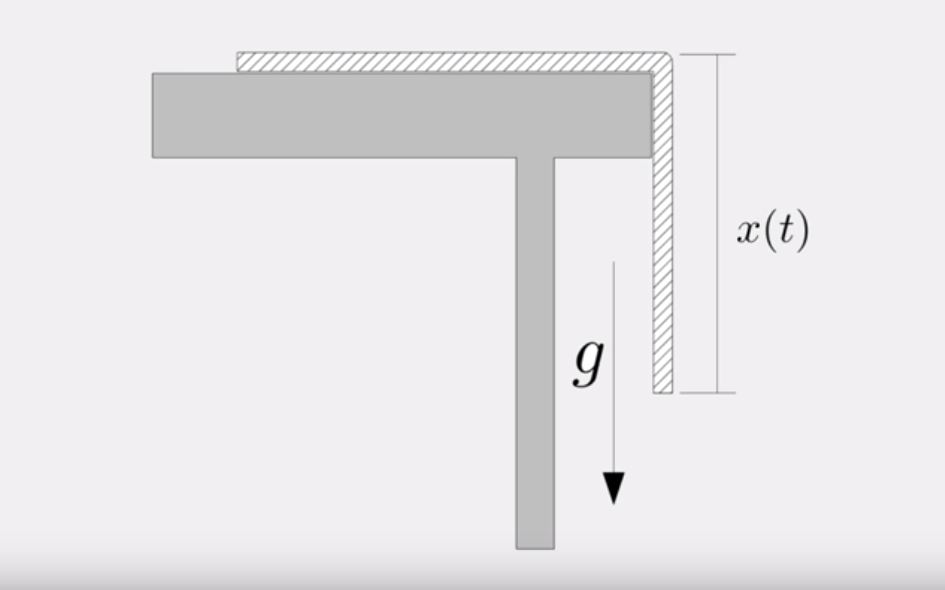
\includegraphics[width=8cm]{ropemass}
		\end{center}
		
	\end{q}
	
	\begin{q}
		\textbf{The Tautochrone} - the curve down which a particle will slide freely under gravity alone, reaching the bottom in time regardless of its starting point on the curve. \\
		A figure of the curve is shown on the side. The starting point is $ P(a,b) $ and the end point is the origin. \\ 
		\begin{center}
			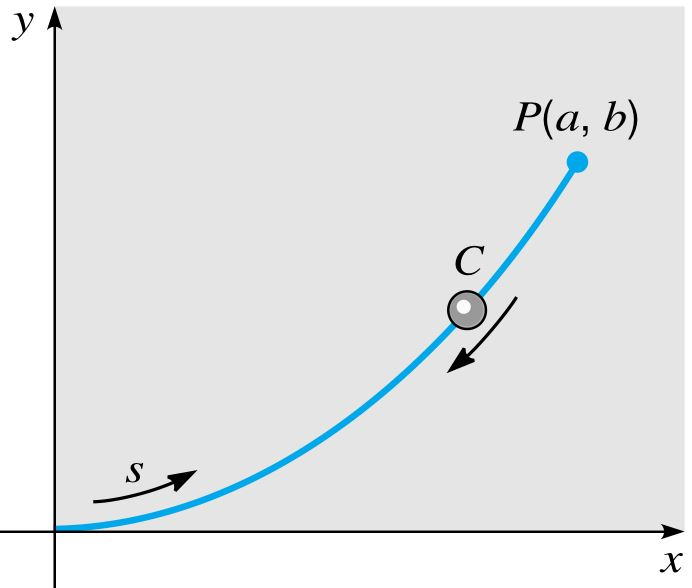
\includegraphics[width=8cm]{taut} 
		\end{center}
		\begin{enumerate}
			\item Given that the Arc length $ s $ is measured from the origin and $ f(y) $ gives the rate of change of $ s $ with respect to $ y $. 
			\[ f(y) = \dfrac{ds}{dy} = \left[1 + \left( \dfrac{dx}{dy} \right)^2 \right]^{1/2} \]
			\item Using conservation of energy the time $ T(b) $ required for a particle to slide from $ P $ to the origin is (Show this step!!)
			\[ T(b) = \dfrac{1}{\sqrt{2g}} \int_{0}^{b}\dfrac{f(y)}{\sqrt{b-y}} dy\]
			\item By the property of a Tautochrone the value of $ T(b) = T_0 $ is a constant for each $ b $. Taking the Laplace transform show that 
			\[ F(s) = \sqrt{\dfrac{2g}{\pi}} \dfrac{T_0}{\sqrt{s}} \] 
			\item Then show that 
			\[ f(y) = \dfrac{\sqrt{2g}}{\pi} \dfrac{T_0}{\sqrt{y}}\] 
			\item Using the previous answers show 
			\[ \dfrac{dx}{dy} = \sqrt{\dfrac{2 \alpha - y}{y}} \]
			where $ \alpha = gT_0^2/\pi^2 $ 
			\item Use the substitution $ y = 2 \alpha \sin ^2 (\theta / 2)$ and show 
			\[ x = \alpha (\theta + \sin \theta) \] \[ y = \alpha (1-\cos \theta)\] 
			Which is a parametric equation of a cycloid, the solution to the problem
		\end{enumerate}
	\end{q}
\end{multicols*}
	\chapter{Systems of First Order Linear Equations}
In this chapter we will skip on reviewing how to solve linear equations, and solve for linear independence. We will only discuss how to solve differential equations using matrices. 
\section{Homogeneous Linear Systems with Constant Coefficients}
We will consider solving functions of the form 
\[ \textbf{x'} = \textbf{Ax} \]
\begin{example}
	Find the general solution of the system 
	\[ 
		\textbf{x'} = 
		\left(
		\begin{matrix}
			2 & 0 \\
			0 & -3 
		\end{matrix}
		\right) \textbf{x}
	 \]
	 Since this is a diagonal matrix we find 
	\[ x_1 ' = 2x_1, \indent x_2' = -3x_2 \]
	The solution for these equations is 
	\[ x_1 = c_1 e^{2t}, \indent x_2 = c_2e^{-3t}\]
	The solutions are 
	\begin{align*}
		\textbf{x}^{(1)}(t) = \left(\begin{matrix}
		1 \\ 0
		\end{matrix}\right) e^{2t} && \textbf{x}^{(2)}(t) = \left(\begin{matrix}
		0 \\ 1
		\end{matrix}\right) e^{-3t}
	\end{align*}
\end{example}
We know that the solution of the equation will be of the form 
\begin{align*}
	\textbf{x} = \xi e^{rt} \\
	r \xi e^{rt} = \textbf{A} \xi e^{rt} \\ 
	\intertext{Upon cancelling the scalar factor, we obtain} 
	(\textbf{A} - r\textbf{I})\xi = \textbf{0}
	\intertext{Where \textbf{I} is the identity matrix  and the solution to this equation is simply the eigenvectors}
\end{align*}
\begin{example}
	\[ \textbf{x}' = \left(\begin{matrix}
		1 & 1 \\ 
		4 & 1 
	\end{matrix}\right) \textbf{x} \]
	Assuming that the solution will be of the form $ \textbf{x} = \xi e^{rt} $ 
	\[ \left(\begin{matrix}
	1-r & 1 \\ 
	4 & 1 -r
	\end{matrix}\right) \left(\begin{matrix}
	\xi_1 \\ 
	\xi_2
	\end{matrix}\right) =  \left(\begin{matrix}
	0 \\ 
	0
	\end{matrix}\right) \]
	We then take the determinant of the matrix on the right side and find $ r^2 - 2r - 3 = (r-3)(r+1) = 0 $. This gives us the eigenvalues, solutions to the equations, $ r =3, -1 $ We then proceed by finding the eigenvectors to the associated eigenvalues 
	\begin{align*}
		\intertext{For when $ r_1 =3 $ we get} 
		\xi^{(1)} = \left(\begin{matrix} 1 \\2\end{matrix}\right)
		\intertext{For when $ r_2 =-1 $ we get} 
		\xi^{(2)} = \left(\begin{matrix} 1 \\-2\end{matrix}\right)
		\intertext{These are the corresponding values to the solution}
		\textbf{x}^{(1)} (t) = \left(\begin{matrix} 1 \\2\end{matrix}\right) e^{3t} && 
		\textbf{x}^{(2)} (t) = \left(\begin{matrix} 1 \\-2\end{matrix}\right) e^{-t} 
	\end{align*}
	The direction field of this system would look like 
	\putpic{model752}
\end{example}
\section{Complex Eigenvalues}
We will now consider the situation where the eigenvalues may be complex numbers. We will return to the form \[ \textbf{x'} = \textbf{Ax} \] where \textbf{A} is the coefficient matrix. The eigenvalues are given by the roots of \[ det(\textbf{A}-r\textbf{I}) = 0\] and that the eigenvectors that satisfy this condition are given by 
\[ (\textbf{A} - r\textbf{I}) \xi = \textbf{0}\] if \textbf{A} is real then the coefficients in the equation are also real, but it is also possible for the roots to appear as a complex number. 
\begin{example}
	Consider th example 
	\begin{align*}
		\textbf{x}' = \left(\begin{matrix}
		-1/2 & 1 \\ 
		-1 & -1/2 
		\end{matrix}\right) \textbf{x} 
		\intertext{making the assumptions we made previously we find that the eigenvalues are}
		r_1 = -1/2 + i && 		r_2 = -1/2 - i 
		\intertext{We find that the corresponding eigenvectors are}
		\xi^{(1)} = \left(\begin{matrix} 1 \\ i \end{matrix}\right), && \xi^{(2)} = \left(\begin{matrix} 1 \\ -i \end{matrix}\right)
		\intertext{Thus the fundamental set of solutions is} 
		\textbf{x}^{(1)} (t) = \left(\begin{matrix} 1 \\i\end{matrix}\right) e^{(-1/2 + i)t} && 
	\textbf{x}^{(2)} (t) = \left(\begin{matrix} 1 \\-i\end{matrix}\right) e^{(-1/2 - i)t}
	\end{align*}
\end{example}
The conditions that help us analyze the complex eigenvalues are such 
\begin{enumerate}
	\item $ \lambda $ have opposite signs; \textbf{x = 0} is a saddle point
	\item $ \lambda $ have same sign but are unequal; \textbf{x = 0} is a node
	\item $ \lambda $ are complex with nonzero real part; \textbf{x = 0} is a spiral point
\end{enumerate}
\section{Fundamental Matrices}
	The structure of the solution of linear differential equations can be furthered using the idea of a fundamental matrix. Suppose that $ \textbf{x}^{(1)}(t)...\textbf{x}^{(n)}(t)$ form a fundamental set of solutions for the equation \[ \textbf{x'} = \textbf{P}(t)\textbf{x} \] Note that the fundamental matrix is nonsingular since its columns are linear independent vectors. 
	\begin{example}
		Find a fundamental matrix for the system \[ \textbf{x}' = \left(\begin{matrix}
		1 & 1 \\ 4 & 1 
		\end{matrix}\right) \textbf{x}\]
		Earlier we found that the set of solutions is 
		\begin{align*}
			\textbf{x}^1 (t) = \left(\begin{matrix}
				e^{3t} \\ 2e^{3t}
				\end{matrix}\right) && 
				\textbf{x}^2 (t) = \left(\begin{matrix}
				e^{-t} \\ -2e^{-t}
				\end{matrix}\right)
		\end{align*}
		are linearly independent so the fundamental matrix is 
		\[ \Psi(t) = \left(\begin{matrix}
				e^{3t} & e^{-t} \\ 2e^{3t} & -2e^{-t}
		\end{matrix}\right) \]
	\end{example}
	Since $ \Psi $ gives the fundamental matrix any multiple by a constant vector will also be a solution. This is expressed as such 
	\[ \textbf{x} = \Psi(t) \textbf{c} \]


	\chapter{Nonlinear Differential Equations and Stability}
So far this concise review has consisted of solving for linear differential equations, because those are the ones that can easily be solved. In this chapter for some reason we will discuss nonlinear equations, but more importantly discuss stability, because that we can qualitatively understand. 
\section{The Phase Plane: Linear Systems}
Lets first begin with a system of the form 
\[ d \textbf{x}/dt = \textbf{Ax} \]
where $ \textbf{A} $ is a $ 2 \times 2 $ matrix and $ \textbf{x} $ is obviously a $ 2 \times 1 $ vector. To review how to solve these differential equations refer to the previous chapter. For now we will consider the \textbf{phase plane} which is the $ x_1x_2 $ plane in which we represent the system above, and the representative set of trajectories of the system is called a \textbf{phase portrait} 
\\ This section is meant to serve as quick summary so here is a table that helps classify and explain what the phase portrait will look like and how we classify its stability
\begin{table}[]
	\centering
	\caption{Properties of Linear Systems $ \textbf{x}' = \textbf{Ax} $}
	\label{that one table}
	\begin{tabular}{@{}lll@{}}
		\toprule
		Eigenvalues & Type of Critical Point & Stability \\ \midrule
		$ r_1 > r_2 > 0 $ & Node & Unstable \\
		$ r_1 < r_2 < 0 $ & Node &  Asymptotically stable\\
		$ r_2 < 0 < r_1 $ & Saddle Point & Unstable \\
		$ r_1 = r_2 > 0 $ & Proper or improper node & Unstable \\
		$ r_1 = r_2 < 0 $ & Proper or improper node & Asymptotically stable \\
		$ r_1, r_2 = \lambda \pm i \mu $ & Spiral point &  \\
		$\lambda > 0$ &  & Unstable \\
		$\lambda < 0$ &  & Asymptotically stable \\
		$ r_1 = i \mu, r_2 = -i\mu  $& Center & Stable \\ \bottomrule
	\end{tabular}
\end{table}
	\\
	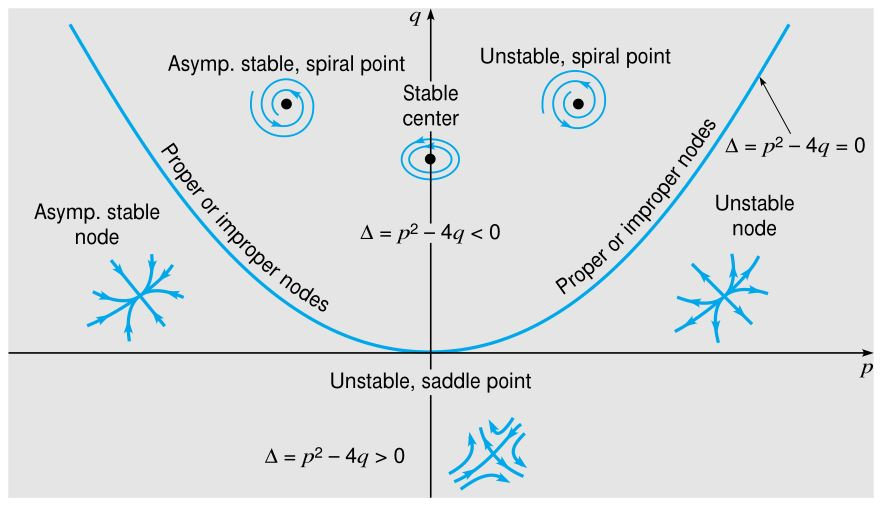
\includegraphics[width=15cm]{phase}
	\\
	Here's a dope diagram, just stare at it for like a long time...  \\
	
	\chapter{Partial Differential Equations and Fourier Series}
This chapter will consider solving problems where the solution is only determined by two boundary values, rather than the initial values we have discussed thus far. Fourier series will also be discussed and how to represent a solutions as the sum of a Fourier series. The Fourier transform will not be discussed, refer to the complex analysis concise review for that information.  
\section{Two Point Boundary Value Problems} 
To begin the section on boundary value problems lets refer back to a familiar form of a second order differential equation 
\[  y'' + p(x)y' + q(x)y = g(x) \] with the boundary conditions \[ y(\alpha) = y_0, \indent y(\beta) = y_1 \] 
Two important terms that are used to classify these differential equations: a problem is classified as \textbf{homogeneous} when the values for $ g $ are always zero and $ y_0 $ and $ y_1 $ are zero as well, otherwise the problem is \textbf{nonhomogeneous}
\begin{example}
	Solve the boundary value problem 
	\begin{align*}
		y'' + 2y = 0, && y(0 ) = 1, \indent y(\pi) = 0
		\intertext{The solution is simply}
		y = c_1 \cos \sqrt{2}x + c_2 \sin \sqrt{2}x 
		\intertext{The first boundary condition requires that the value for $ c_1 $ be equal to $ 1 $ the second boundary condition requires that $ c_2 $  be equal to $ -\cot \sqrt{2} \pi $. Thus the solution to differential equation is}
		y = \cos \sqrt{2}x - \cot \sqrt{2}\pi \sin \sqrt{2}x 
		\intertext{This is an examples of a case where the solution is unique and the problem is nonhomogeneous}
	\end{align*}
\end{example}
\begin{example}
	Solve the boundary value problem 
	\begin{align*}
	y'' + y = 0, && y(0)=1, \indent y(\pi)=a \\
	\intertext{where a is a given number} 
	\intertext{The general solution of this differential equation is}
	y = c_1 \cos x + c_2 \sin x 
	\intertext{From the first boundary condition we find that $ c_1 =1  $. The second boundary condition now requires that $ -c_1 = a $. These two conditions on $ c_1 $ are incompatible if $ a \neq -1 $, so the problem has no solution in this case. if $ a = -1 $ then both boundary conditions are satisfied for  }
	\end{align*}
\end{example}
\end{document}